\section{Introduction}

% With the advent of reasonably large labeled datasets such as the VGMIDI dataset \cite{ferreira_2019}, it became feasible to investigate AAC \cite{williams2015investigating} as a problem of steering the probability distribution of neural LMs towards a target emotion. Given a neural LM $L$, a prior sequence of music tokens $x = [x_1, \dots, x_{t-2}, x_{t-1}]$, a target emotion $e$, and a music emotion classifier $E$, the problem consists of decoding the $L$'s output layer to predict the next tokens $x' = [x_t, x_{t+1}, \cdot, x_n]$ with the guidance of the classifier $E$ in order to maximize the likelihood of $x'$ having the target emotion $e$.

% The previous chapter presented SBBS, a decoding strategy that approaches this problem based on the beam search algorithm.
This chapter presents a new decoding strategy based on Monte Carlo Tree Search (MCTS) to generate musical pieces conveying a target emotion. Similar to SBBS, MCTS uses a music emotion classifier $E$ to steer the probability distribution of a neural LM $L$ towards a target emotion $e$ at generation time. Unlike SBBS, MCTS performs multiple search iterations for each decoded token. Each iteration uses the Predictor Upper Confidence for Trees (PUCT) to update the distribution of node visits $N$, where $E$ determines the expected reward (\textit{Q value}) of each node and $L$ the prior probability of selecting each node (\textit{P value}). After all the search iterations to decode the next token, $N$ ends up steering $L$ towards $e$. Therefore, the next token is decided by sampling from $N$.

The search is performed over the space of sequences learned by a music transformer LM \cite {huang2018music} with the unlabelled pieces of the VGMIDI dataset. The number of unlabelled pieces of the VGMIDI dataset has been extended as part of this work from 728 to 3,640. Similar to the approaches presented in Chapter \ref{ch:ismir19} \cite{ferreira_2019} and Chapter \ref{ch:aiide20} \cite{ferreira2020computer}, the music emotion classifier is trained by fine-tuning a pre-trained LM with a classification head on the 200 labeled pieces of the VGMIDI dataset. Unlike these two previous approaches, emotion classification is treated as a multiclass problem instead of a binary one. In this new framing, each of the four quadrants of the circumplex model is mapped to a label.

MCTS is evaluated with two listening tests, one to measure the quality of the generated pieces and one to measure MCTS's accuracy in generating pieces with a target emotion. In the first test, human subjects are asked to prefer between MCTS, the validation data (human compositions), TopK sampling, and SBBS \cite{ferreira2020computer}. In the second test, human subjects are asked to annotate the emotions they perceive in pieces generated by MCTS, TopK sampling, and SBBS. Results show that MCTS outperforms SBBS in terms of music quality while slightly improving the accuracy of conveying target emotions. MCTS and TopK performed similarly in terms of music quality. An expressivity analysis \cite{smith2010analyzing} is performed to evaluate how MCTS conveys each target emotion. The frequencies of pitch classes and note durations suggest that MCTS can reproduce some common composition practices used by human composers.

% \section{Language and Emotion Models}

% In this section we describe the language and emotion models used to guide the generation of music with perceived emotion.

\section{Language Model}

Music transformer \cite{huang2018music} is currently one of the state-of-the-art NN architectures for symbolic music generation, and hence it is used to train a base LM for MCTS. This LM is trained on the unlabelled pieces of the VGMIDI dataset. Originally, the VGMIDI dataset had 728 unlabelled pieces, but it has been expanded to 3,640 pieces in this work. The new pieces are piano arrangements of video game music created by the NinSheetMusic community\footnote{\url{https://www.ninsheetmusic.org/}}. The VGMIDI dataset has been used, instead of other large datasets of symbolic music (e.g., the MAESTRO dataset \cite{hawthorne2018enabling}), to be able to train both the LM and the music emotion classifier on similar datasets.

The VGMIDI pieces are encoded using a different vocabulary than the original one proposed with music transformer \cite{huang2018music}. Aiming at reducing the length of the music sequences, the MIDI files are mapped to sequences using a large expressive vocabulary instead of a compact one. To create a sequence from a MIDI file, the starting times of all the notes are discretized into a sequence of time steps. Then, each time step is processed in order, generating a token $n_{p, d, v}$ for each note in the time step. The three parameters of a note token $n_{p, d, v}$ are pitch $p$, duration $d$ and velocity $v$, respectively. In order to constrain the possible combinations of note tokens, the pitch values are limited to $30 \leq p \leq 96$. Duration $d$ is limited by the types: breve, whole, half, quarter, eighth, 16th and 32nd. The dotted versions of these types (maximum of 3 dots) are also considered. Velocities are limited to the values $v \in [32, 36, 40, \cdots, 128]$. After processing each time step, a token $r_d$ is generated representing a rest with a given duration $d$. The token ``$.$'' (period) is included at the end of all time steps to represent the end of the piece.

This encoding scheme yields a vocabulary with 44,346 tokens, which is orders of magnitude larger than the vocabularies described in Chapters \ref{ch:ismir19} (225 tokens) and \ref{ch:aiide20} (314 tokens). The benefit of this large vocabulary over the small ones described previously is that it allows the MIDI files to be mapped to considerably smaller sequences. Music transformer networks can only process sequences with a fixed size. Thus, reducing the size of the encoded pieces allows the music transformer to model pieces entirely and hence capture long-term dependencies in music. Moreover, according to \citet{holtzman2018learning}, LMs with larger vocabularies tend to generate less repetitive sequences. On the other hand, by having more tokens, MCTS has more options to choose from at any given point of the generative process, which increases the search complexity. MCTS mitigates the effects of having more options to choose from by only considering the top $k$ tokens according to the LM at any decision point of the generative process.

% In this work, the probability of a sequence of tokens $s$ according to the LM is denoted as $L(s)$ and the probability of the sequence $s$ added of the token $l$ as $L(s, l)$.

\section{Music Emotion Classifier}
\label{sec:emotion_classifier}

In chapters \ref{ch:ismir19} and \ref{ch:aiide20}, it has been shown that fine-tuning a LM with an extra classification head yields a better model than training a classifier from scratch with the same architecture of the LM. This work follows a similar approach. The Music Transformer LM described in the previous section is fine-tuned as a music emotion classifier with the labeled pieces of the VGMIDI dataset. In chapters \ref{ch:ismir19} and \ref{ch:aiide20}, symbolic music emotion classification is approached as two independent binary problems, one for valence and one for arousal. This work defines it as a multiclass problem. Four emotions are considered: high valence and arousal (E0), low valence and high arousal (E1), low valence and arousal (E2), and high valence and low arousal (E4). Each labeled piece in the VGMIDI dataset has a valence label $v \in [-1, 1]$ and an arousal label $a \in [-1, 1]$. A pair of values is mapped to a categorical label (E0, E1, E2, or E3) by getting the quadrant of $(v,a)$. As shown in Figure \ref{fig:va_mapping}, a piece with values $(1,1)$ is mapped to E0, $(-1,1)$ to E1, $(-1,-1)$ to E2, and $(1, -1)$ to E3.

\begin{figure}
 \centering
 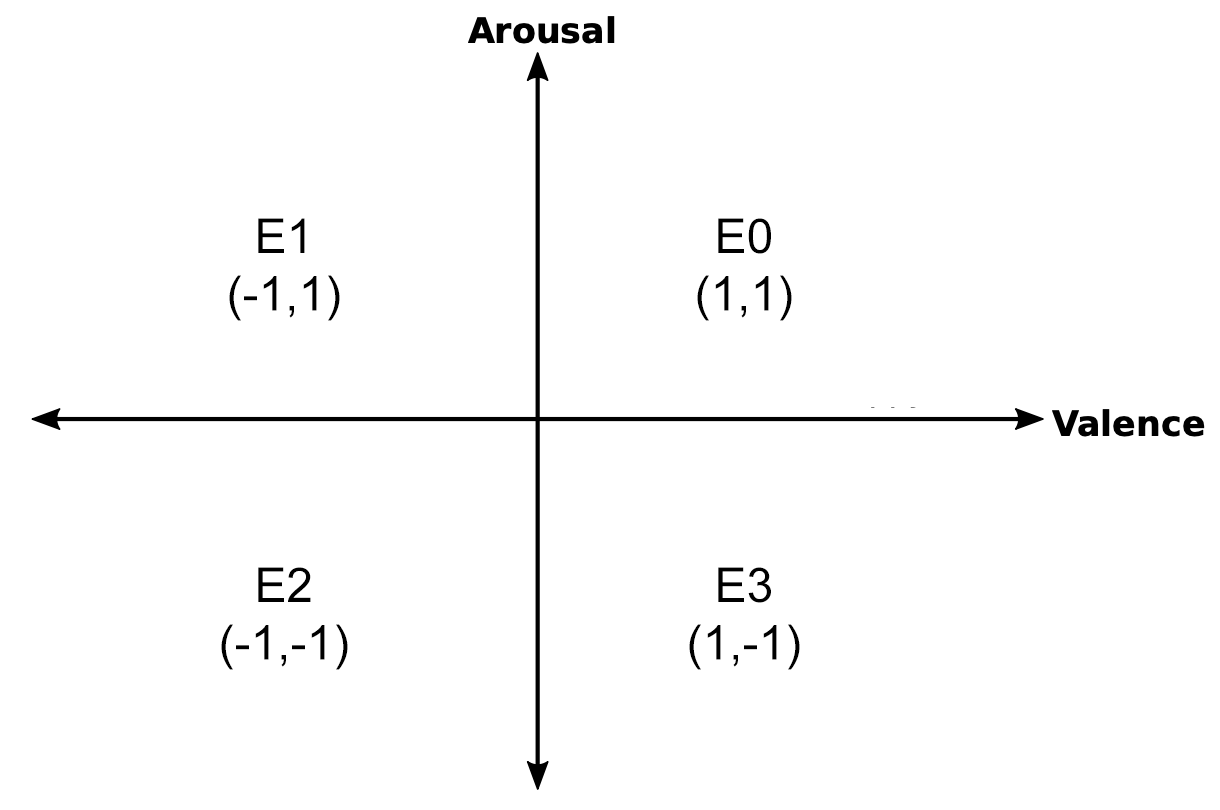
\includegraphics[width=0.7\columnwidth]{imgs/ismir21/circumplex.png}
 \caption{Mapping the circumplex model to a categorical model of emotion with four classes: E0, E1, E2, and E3.}
 \label{fig:va_mapping}
\end{figure}

This mapping yields 76 pieces with label E0, 38 with label E1, 27 with label E2, and 59 with E3. This multiclass approach is used to simplify the search task of controlling the emotion of the generated pieces: only a single model defines the emotion scores instead of a combination of two models. Since MCTS evaluates the emotion of sequences with different lengths (see Section \ref{sec:puct}), the music emotion classifier is trained with prefixes of different lengths extracted from the labeled pieces. Thus, during training, the classifier learns a mapping of a sequence to an emotion considering different lengths. This is especially helpful to guide the search at the beginning of the generation process, where the number of generated tokens is short, and so the emotion classifier does not have much context to be confident about a prediction.

% In this work, $E$ denotes the emotion model and $E(s, e)$ the probability of a sequence $s$ being perceived as a piece of emotion $e$.

\section{MCTS for Music Generation}
\label{sec:puct}

% MCTS
Monte-Carlo Tree Search (MCTS) is a heuristic search algorithm traditionally used to play board games with large search spaces. Before taking an action at the current game state, MCTS iteratively explores the branches of the search tree, looking ahead to determine how different game moves could lead to stronger or weaker states of the game. MCTS variations use a variety of algorithms for deciding which branches of the tree to explore next. For example, UCT \cite{Kocsis2006} uses the UCB1 formula for deciding which branches to expand in each iteration of the algorithm, while AlphaZero uses the PUCT formula \cite{silver2017mastering}. This section describes how this work employs PUCT to generate music with a specific target emotion.

PUCT receives a sequence $x = \{x_1, x_2, \cdots, x_{t-1}\}$ of musical tokens as input, which will bias the generative process; a music emotion classifier $E$; a language model $L$; a parameter $k$ defining the number of top tokens (according to $L$) to consider when deciding the next token; a parameter $d$ defining the number of search iterations PUCT can perform before deciding the next token; and a target emotion $e$. PUCT returns a sequence $x'$ with prefix $x$ for which $E(x', e)$ and $L(x')$ are maximized. PUCT grows a search tree where each node $n$ represents a sequence of tokens from the vocabulary. The root of the tree represents the prefix $x$ provided as input. Each edge $(n, m)$ from node $n$ to node $m$ represents the addition of a token to the sequence $n$ ($m$ is one token larger than $n$). In this formulation, $m$ is called a child of $n$, and since each node $n$ represents a sequence $x$, $n$ and $x$ are used interchangeably. Initially, PUCT's tree is of size one as it only contains the root of the tree. In each iteration, PUCT performs the following steps to add a new node to the tree: (1) \textbf{selection}, (2) \textbf{expansion}, (3) \textbf{simulation}, and (4) \textbf{backpropagation}.
% We explain each of these steps and their intuition.

\begin{enumerate}
    \item \textbf{Selection}

    Starting from the current node $n$, PUCT recursively selects the token $l$ that maximizes Equation \ref{eq:puct} until $l$ leads to a node $m$ that is not in the PUCT tree. In Equation \ref{eq:puct}, $Q(n, l)$ is the expected emotion ``reward'' of the sequence $(n, l)$ as given by $E$, $c$ is an exploration constant, $P(n, l)$ is the prior probability of $l$ being the next token from $n$ as given by $L$, $N(n)$ is the number of times node $n$ has been visited in the selection step, and $N(n, l)$ is the number of times token $l$ has been chosen from node $n$ in a selection step.

    \begin{equation}
    \argmax_{l} Q(n, l) + c \times P(n, l) \times \frac{\sqrt{N(n)}}{1 + N(n, l)}
    \label{eq:puct}
    \end{equation}

    In practice, only the $k$ tokens with the largest probability according to $L$ are considered in the selection step. This allows PUCT to focus on the sequences that are more promising according to the LM.

    \item \textbf{Expansion}

    The node $m$ returned in the selection step is then added to the PUCT tree and its statistics are initialized: $N(m) = 1$, $N(m, l) = 0$, and $Q(m, l) = 0$ for all top $k$ tokens $l$ according to the probability $L(m, l)$.

    \item \textbf{Simulation}

    The recently added node $m$ is evaluated according to the target emotion $e$. The $Q(n, l)$-value (recall that adding $l$ to $n$ generated the node $m$) is given by $E(m, e)$. The value of $N(n, l)$ is set to $1$ as this is the first time $l$ is selected from node $n$.
    %Inspired in the scheme employed in AlphaZero~\cite{alphazero},
    %instead of adding symbols to the sequence node $n'$ represents until reaching an end-of-music symbol,
    %we use $E(n', e)$ as the $Q(n, l)$-value.

    \item \textbf{Backpropagation}

    The value of $Q(n, l)$ is used to update the $Q$-values of all the other node-token pairs recursively selected in the \textbf{selection step}. This is achieved by following the path in the tree from $n$ to $m$ in reverse order and updating the statistics of each node $n$ in the path according to Equation \ref{eq:puct_backprop}.

   \begin{align}
   \label{eq:puct_backprop}
   \begin{split}
   Q(n, l) &= \frac{Q(n, l) \times N(n, l) + E(m, e)}{N(n, l) + 1} \\
   N(n, l) &= N(n, l) + 1 \\
   N(n) &= N(n) + 1
   \end{split}
   \end{align}

   The $Q(n, l)$-values are the average $E$-values of the sequences with prefix given by $n$. In other words, the value of $Q(n, l)$ is the average emotion ``reward'' of the sequences with the prefix given by $n$. The backpropagation step completes an iteration of PUCT.

\end{enumerate}

In the next iteration, PUCT will perform the four steps described above, but with updated values of $N$ and $Q$ for the node-token pairs selected in the previous iteration. Equation \ref{eq:puct} guarantees that the sequences $n$ that maximize the value of $E(n, e)$ are visited more often as they will have larger values of $Q$. The PUCT formula also accounts for the probability given by the language model, giving preference to sequences with higher probability according to $L$. Finally, the term $\frac{\sqrt{N(n)}}{1 + N(n, l)}$ certifies that all nodes have a chance of being explored by the search.
%allows even nodes that are considered unpromising by the language and emotion models to be explored by the search.

PUCT performs $d$ iterations before deciding which token will be added to the sequence represented at the root of the tree. That is, the search budget of $d$ iterations is to decide the next token of the sequence. Let $n$ be the root of the tree. The token $l$ that will be added to the sequence $n$ is sampled from the distribution given by the values $\frac{N(n)}{\sum_{l} N(n, l)}$. The node $m$ resulting from the addition of $l$ to $n$ becomes the new root of the tree and another PUCT search is performed with budget $d$ to choose the next token to be added to $m$. This process is repeated until a desired number of tokens are generated. The PUCT search can be seen as an operator that changes the probability distribution over tokens given by the language model such that it accounts for the target emotion. This is because the distribution given by $\frac{N(n)}{\sum_{l} N(n, l)}$ will favor tokens that lead to pieces matching the target emotion as nodes representing such pieces are visited more often during search.

\section{Empirical Evaluation}

MCTS is evaluated with two listening tests, one for measuring the quality of the generated pieces and one for measuring the accuracy of MCTS in conveying a target emotion. All experiments are performed via Amazon Mechanical Turk (MTurk). For both experiments, MCTS is compared against SBBS, TopK sampling, and human-composed pieces. Although TopK sampling does not consider emotion, it is a good baseline for music quality. MCTS is not compared against the approach from Chapter \ref{ch:ismir19} because that approach is limited to sentiment. To generate the pieces to be evaluated, 10 prime sequences are selected from the VGMIDI dataset for each of the 4 emotions. Each prime sequence is then used to generate a piece with each of the 4 models, yielding $10\times4\times4 = 160$ pieces. Each piece has 512 tokens. Each prime sequence is 32 tokens long and is selected at random from the VGMIDI test set with the target emotion $e$. For the human method, pieces are ``generated'' by simply extracting the first 512 tokens of the piece with the given prime.

To generate the 160 pieces, a Music Transformer LM is first trained with 4 layers (transformer blocks), a maximum sequence length of 2048 tokens, 8 attention heads, and an embedding layer with 384 units. The size of the Feed-Forward layers in each transformer block is set to 1024. This music transformer LM is trained with the 3,640 unlabelled pieces of the extended VGMIDI dataset, where 3,094 (85\%) of the pieces are used for training and 546 (15\%) for testing. All unlabelled pieces are augmented by (a) transposing to every key, (b) increasing and decreasing the tempo by 10\%, and (c) increasing and decreasing the velocity of all notes by 10\% \cite{oore2017learning}. The emotion classifier is then trained by fine-tuning the music transformer LM with an extra linear classification layer on top. The emotion classifier is trained with the 200 labeled pieces of the VGMIDI dataset, where 140 (70\%) pieces are used for training and 30 (30\%) for testing. After training, the losses of the music transformer LM are 0.54 on the training set and 0.73 on the test set. The accuracy of the emotion classifier on the test set is 61\%. At generation time, the LM distribution is filtered with $k = 128$ in MCTS, SBBS, and TopK. The beam size for SBBS is set to $b = 4$. For MCTS, the number of simulation steps is set to $d = 30$ and the exploration constant to $c = 16$.

% TODO: add prefixes sizes

\subsection{Quality Listening Test}

The quality listening test consists of a pairwise comparison that follows the methodology proposed by \citet{huang2018music}. Human subjects were presented with two generated pieces from two different models that were given the same priming sequence. The two pieces were presented side-by-side, and the participants were asked to select which one is more musical using a 5-point Likert scale. In this scale, 1 means "Left piece is much more musical", 2 means "Left piece is slightly more musical", 3 means "Tie", 4 means "Right piece is slightly more musical" and 5 means "Right piece is much more musical". The order of the two pieces was randomized to avoid ordering bias. Each of the 240 pairs of generated pieces were evaluated by 3 MTurk workers. In order to reduce noise in the results (mainly caused by random choices in Amazon MTurk), a test evaluation is included for each human subject. This test is another pair of pieces to be evaluated with the same Likert scale, but one piece is a human-composed piece and the other one is sampled from the LM without TopK filtering and temperature equal to 1.5 (forcing the sample to have poor quality). The subjects are also asked to briefly justify their choice with 1-3 short sentences. Participants who failed the test evaluation (choosing the sampled piece as more musical) or didn't write explanations longer than 5 words were filtered out. In total, this experiment yielded 389 comparisons. Each pair was evaluated at least once.

Table \ref{tab:quality} shows the results of the quality test. The top part of the table shows the number of wins, ties, and losses of one model against another.  MCTS performed exactly like TopK sampling and outperformed SBBS by ten wins. Surprisingly, MCTS won against human-composed pieces 12 times and tied 9 times. SBBS performed worse than TopK sampling, winning 26 times and losing 31. As expected, all models performed worse than human compositions. The bottom part of the table shows the percentage of wins, ties, and losses for one model against all other models. Percentages are reported because, due to the filtering of the participants, the amount of comparisons for each model is not the same. The aggregated results also show that MCTS performs better than SBBS and the same as TopK sampling. A Kruskal-Wallis H test of the subject choices (values from 1 to 5) shows a statistically significant difference between the models with $p = 1.5e-4 < 0.01$.

% TODO: Run statistical tests
\begin{table}[h]
    \centering
    \begin{tabular}{ccccc}
    \toprule
   \multicolumn{2}{c}{\textbf{One-Vs-One}} & \textbf{Wins} & \textbf{Ties} & \textbf{Losses} \\
    \midrule
    \textbf{MCTS} & \textbf{TopK } & 25 & 13 & 25 \\
    \textbf{MCTS} & \textbf{SBBS } & 34 & 8  & 24 \\
    \textbf{MCTS} & \textbf{Human} & 12 & 9  & 41 \\
    \textbf{TopK} & \textbf{SBBS } & 31 & 6  & 26 \\
    \textbf{TopK} & \textbf{Human} & 15 & 7  & 45 \\
    \textbf{SBBS} & \textbf{Human} & 15 & 8  & 45 \\
    \midrule
    \multicolumn{2}{c}{\textbf{One-Vs-Rest}} & \textbf{Wins \%} & \textbf{Ties \%} & \textbf{Losses \%}  \\
    \midrule
    \multicolumn{2}{c}{\textbf{MCTS}} & 38 & 15 & 47  \\
    \multicolumn{2}{c}{\textbf{SBBS}} & 33 & 12 & 55  \\
    \multicolumn{2}{c}{\textbf{TopK}} & 37 & 13 & 50 \\
    \multicolumn{2}{c}{\textbf{Human}} & 66 & 12 & 22 \\
    \bottomrule
    \end{tabular}
    \caption{Results of the quality listening test. The top part of the table reports the number of wins, ties, and losses for a model against each other model. The results are stated with respect to the left model. For example, MCTS won against SBBS 34 times and lost to SBBS 24 times. The bottom part of the table shows the percentage of wins, ties, and losses for a model against all the others.}
    \label{tab:quality}
\end{table}

\subsection{Emotion Listening Test}

In the emotion listening test, human subjects were asked to annotate the generated pieces according to the circumplex model of emotion using the same tool designed to annotate the VGMIDI dataset (see Section \ref{sec:data_collection}). An annotation result is a time series of valence-arousal pairs where each element corresponds to a chunk (a bar if the piece has 4/4 time signature) of the piece. For this experiment, 3 MTurk workers were assigned for each piece generated by the MCTS, SBBS, and TopK methods (total of 360 annotations). Human pieces are not reannotated because they are the ground truth data used to train the music emotion classifier that is base for both MCTS and SBBS. No annotations were filtered out in this experiment.

The accuracy of a method in conveying a target emotion is measured with the percentage of chunks in the annotations that match the target emotion. Each valence-arousal pair is mapped to an emotion label by getting the quadrant of that valence-arousal pair (see Section \ref{sec:emotion_classifier} for details).  Table \ref{tab:emotion} reports the accuracy of each model for each emotion. Overall, MCTS outperformed TopK (no emotion control) by an average of 15\%. MCTS performed similarly to SBBS, with slightly better average accuracy. It is important to highlight that MCTS was able to considerably improve the accuracy in conveying the two least represented emotions (E1 and E2) in the VGMIDI dataset. This is a great result since labelling symbolic music according to emotion is an expensive task.

% TODO: Add standard deviation
\begin{table}[h]
    \centering
    % \setlength{\tabcolsep}{4pt}
    \begin{tabular}{cccccc}
    \toprule
    \textbf{Model} & \textbf{E0} & \textbf{E1}  & \textbf{E2} & \textbf{E3} & \textbf{Avg.} \\
    \midrule
    \textbf{MCTS} & \textbf{72} & \textbf{52} & \textbf{37} & 57 & \textbf{54} \\
    \textbf{SBBS} & 67 & 41 & 30 & \textbf{70} & 52 \\
    \textbf{TopK} & 61 & 18 & 26 & 53 & 39 \\
    \bottomrule
    \end{tabular}
    \caption{Accuracy of each model in conveying the target emotions E0, E1, E2 and E3. }
    \label{tab:emotion}
\end{table}

TopK performed reasonably well on average (39\%), but this was primarily due to its ability to convey the two most represented emotions in the training data (E0 and E3). These two emotions are very likely more represented in the unlabelled data as well, which was used to train the LM. Even though TopK sampling does not control emotion, the prime sequences they used to generate the pieces had the target emotions. Therefore, TopK (like all other models) is conditioned with this prime sequence towards the desired emotion. However, because TopK does not consider emotion when generating pieces, eventually it starts sampling tokens that deviate from the target emotion.

The three models performed poorly on conveying E2, which encompasses basic emotions such as sad, depressed, and tired. These poor performances can be explained by the fact that class E2 has the least number of examples in the VGMIDI dataset. Moreover, as showed in Chapter \ref{ch:ismir19}, negative pieces can be considered ambiguous by human annotators. One could mitigate this problem by increasing the number of pieces of class E2 in the VGMIDI dataset.

Although MCTS performed similarly to SBBS in terms of emotion, MCTS outperformed SBBS considerably with respect to music quality. SBBS tends to generate repetitive pieces more often than MCTS once repetition maximizes both the probabilities of the LM and the music emotion classifier. Since SBBS does not do backtracking, when it generates a good pattern that is likely according to the LM and that conveys the target emotion, it tends to repeat that pattern. Figure \ref{fig:ex_pieces} illustrates this problem with examples of pieces generated by MCTS and SBBS. These two pieces were given the same prime sequence \footnote{Note that the first 8 seconds of the two pieces are the same.} $x$ with the target emotion E2 (low valence and arousal). MCTS developed $x$ by creating 4 parts: an introduction from $t=0$ to $t=15$, a \textit{Part A} from $t=15$ to $t=30$, a \textit{Part B} from $t=30$ to $t=43$, and a \textit{Part C} from $t=43$ until the end. Parts A, B, and C are similar to each other but present different variations of the bass line presented in the last 3 seconds of the introduction. SBBS, on the other hand, simply repeated the bass line and the chord presented in $x$ until the end of the piece. This is a case where SBBS repeated a given pattern that maximized the LM and the music emotion classifier probabilities. This example also shows how backtracking allows MCTS to look for different patterns in the search space.

\begin{figure}[h]
\centering
 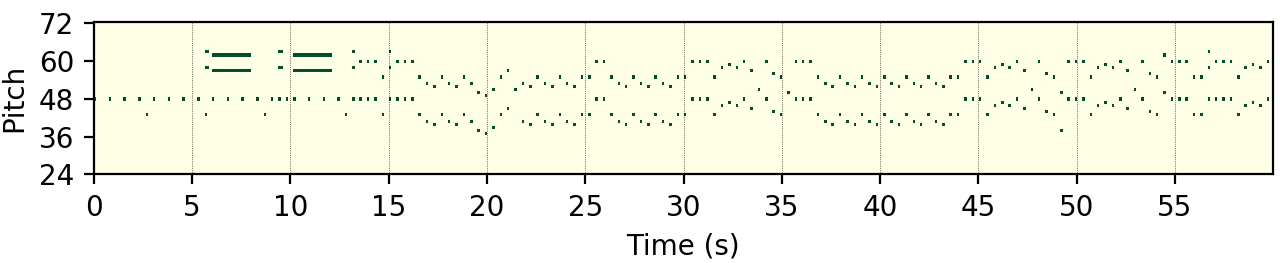
\includegraphics[width=\columnwidth]{imgs/ismir21/mucts_piece_2_14.png}
 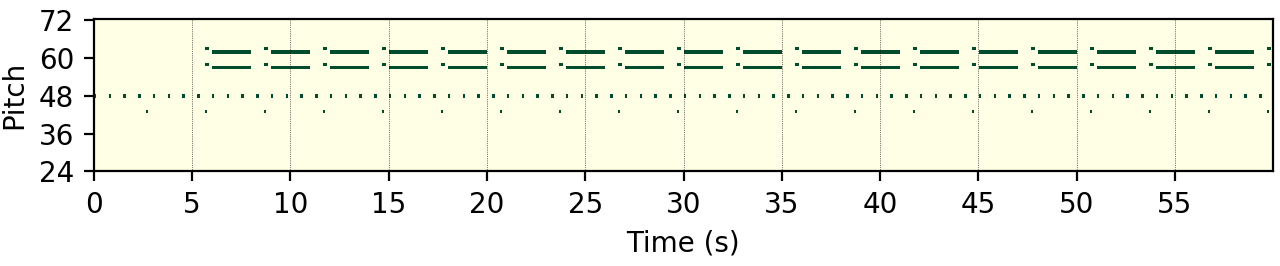
\includegraphics[width=\columnwidth]{imgs/ismir21/sbbs_piece_2_14.png}
 \caption{Examples of MCTS (top) and SBBS (bottom) pieces controlled to have emotion E2.}
 \label{fig:ex_pieces}
\end{figure}

\section{Expressivity Range}

An expressivity analysis is performed to better understand how MCTS conveys different target emotions. Expressivity analysis is an evaluation method commonly used in the AI and Games research community to compare different level generators \cite{smith2010analyzing}.  It consists of generating a large set of levels and measuring the biases of the generators according to pre-defined relevant metrics. In the music generation domain, this approach is used to explore the biases of the MCTS generator when conveying each emotion with respect to human compositions.

% TODO: Compare with human expressivity (maybe run a statistical tests)
The expressivity analysis is performed on the 40 pieces generated by MCTS for the previous experiments, considering the frequencies of pitch classes and note durations as the metrics to measure bias. Figure \ref{fig:expressivity} illustrates the distribution of pitch classes and note durations for both MCTS and human-composed pieces. Overall, the MCTS and human distributions of note durations look similar. For label E0 (high valence and arousal), human pieces predominantly have 16th notes, but a few 8th notes are also present. Quarter notes and 32nd notes are rarely used. MCTS also explored mainly 16th notes for label E0, however it used considerably more 8th and 32nd notes than the human compositions. Label E0 encapsulates emotions such as happy, delighted, and excited. These results show that both VGMIDI pieces and MCTS generated pieces with these emotions have rhythm patterns with shorter notes.
% In terms of pitch classes, MCTS used mainly C, C\#, D, E, and A to control pieces in E0.

% TODO: discuss pitch usage
\begin{figure}[h]
\centering
 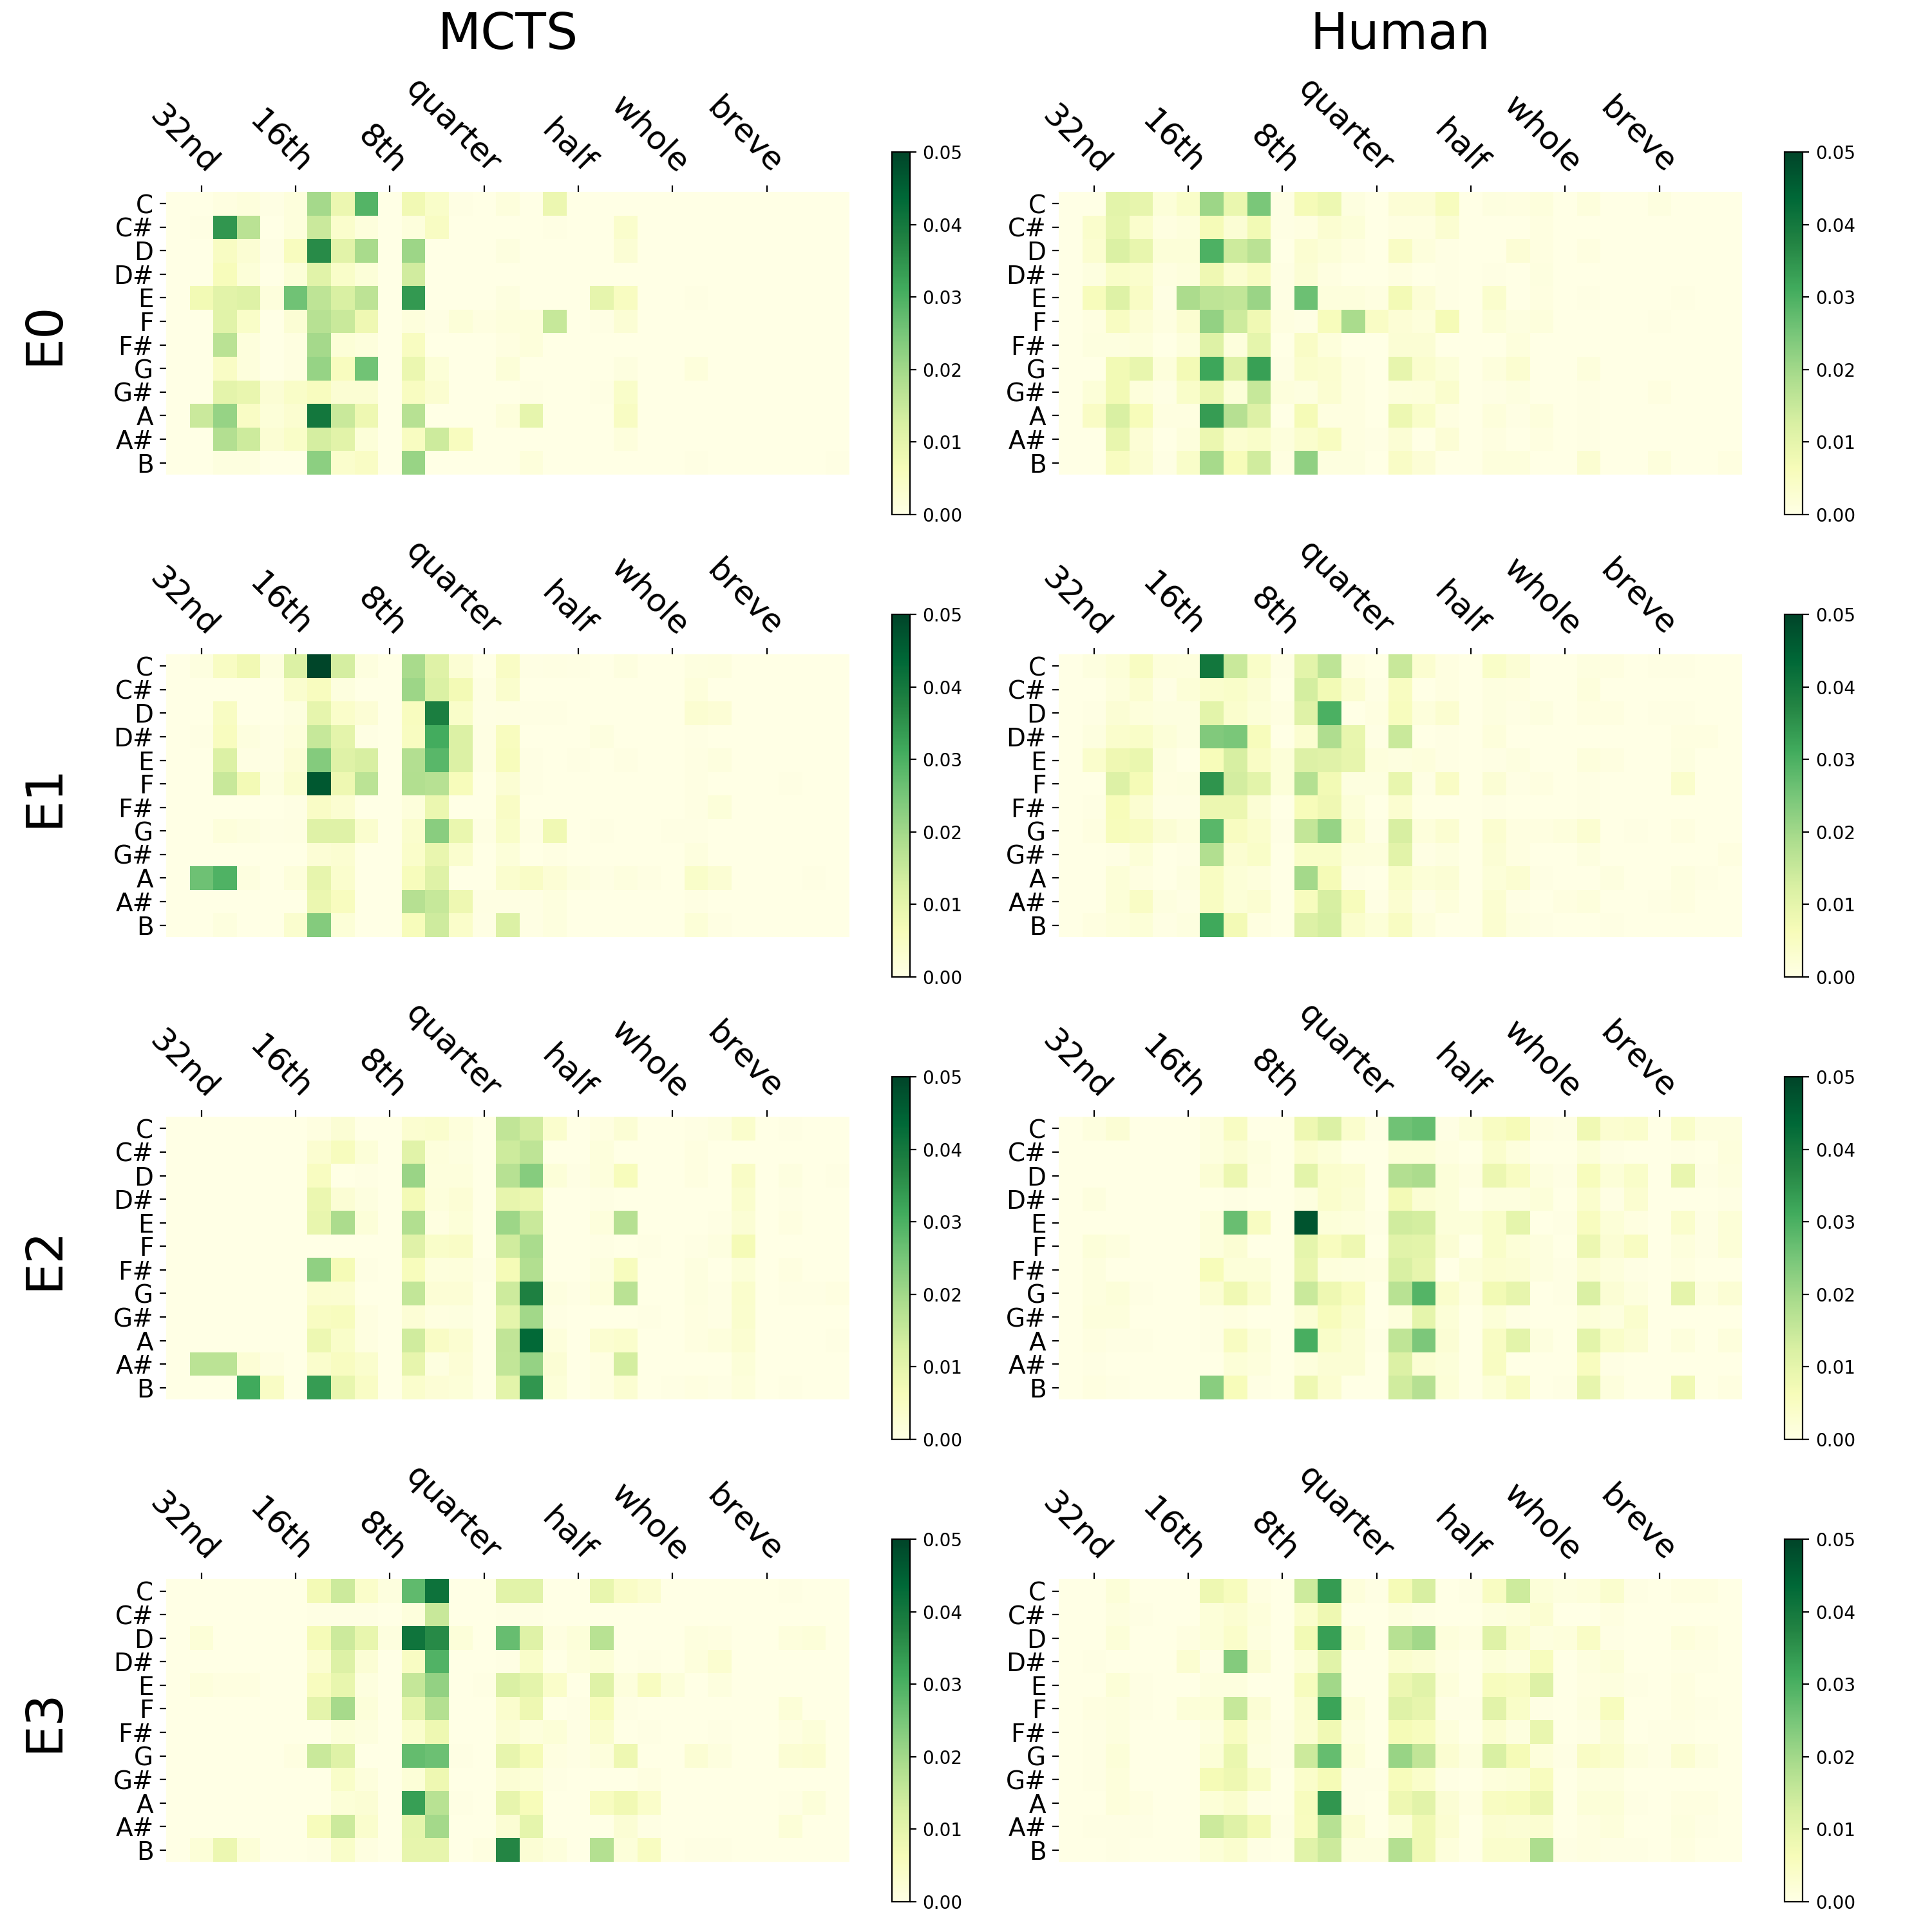
\includegraphics[width=0.8\columnwidth]{imgs/ismir21/mcts_human.png}
   \caption{MCTS expressivity range. The x axis represents note duration in seconds and the y axis represents pitch classes. }
 \label{fig:expressivity}
\end{figure}

For label E1 (low valence and high arousal), human compositions have a more even distribution between 16th and 8th notes. Quarter notes are present but with a relatively low frequency, and 32nd notes are rarely used. MCTS also used a combination of 16th and 8th notes, but it used fewer quarter notes and a little more 32nd notes than the human compositions. Label E1 represents emotions such as tense, angry, and frustrated. Combining these results with the expressivity range of label E0, one concludes that the VGMIDI and MCTS pieces with high valence have rhythm patterns with notes shorter than a quarter note.

For label E2 (low valence and arousal), human pieces are mainly composed of quarter notes, with a few 8th and 16th notes. Different than E0 and E1, E2 has a few long notes such as half, whole, and breve notes. MCTS also focused on quarter notes for label E2. However, MCTS used more short notes and fewer long notes than human compositions. Label E2 encapsulates emotions such as sad, depressed, and tired. According to these results, both human and MCTS pieces with these emotions tend to have rhythm patterns with long notes.

% This is also an expected result since  Music in this space tends to have a slow tempo and rhythm patterns with long notes. For E2, the pitch classes G, A, and B were the most frequent ones.

For label E3 (high valence and low arousal), both human and MCTS pieces have mainly 8th notes with a few 16h, quarter, and whole notes. These pieces represent emotions such as calm, relaxed, and content. With these expressivity results, one concludes that pieces with low arousal have rhythm patterns with long notes.

% In video game music, Calm music (such as the "Sims" theme) tends not to be very slow once the game wants to keep the player engaged. Thus, having this wide combination of durations centered around dotted 8th notes seems a good choice.

\section{Conclusions}

This chapter presented a decoding algorithm based on MCTS to generate symbolic music with controllable emotion. MCTS used PUCT to explore the search tree, where the probability of the nodes comes from a LM, and their scores are given by a music emotion classifier. MCTS was evaluated with two listening tests, one to measure the quality of the generated pieces and one to measure the accuracy of MCTS in conveying target emotions. In the first experiment, a pairwise comparison is performed between pieces generated by MCTS, SBBS, TopK sampling, and human composers. Human subjects were asked to rate which pieces they found more musical. In the second experiment, human subjects annotated the emotions they perceived in the generated pieces. Results showed that MCTS outperforms SBBS in terms of quality and has slightly better accuracy when controlling emotions. With an expressivity analysis, it was shown that MCTS generates pieces with music features similar to human compositions.

This is the first work to apply MCTS to decode neural LMs to generate symbolic music with controllable emotion. Given that MCTS is agnostic to the classifier used to steer the distribution of the LM, it can be used to control different features as long as a classifier can discriminate those features. Since MCTS generates music by searching over a large vocabulary with approximately 45K tokens, its generative task is similar to other NLP generative tasks. Therefore, MCTS can also be generalized to decode and control LMs in text generation tasks.
